% !TEX program = xelatex
% ============================================================================
%  POSN Computer Qualification — Circles
%  Topic: วงกลม (Circles)
% ============================================================================

\documentclass[11pt, aspectratio=169]{beamer}
% ============================================================================
%  POSN Computer Qualification — Shared Beamer Preamble
%  Used by all topic slide decks. Compile with XeLaTeX.
% ============================================================================

% ---------- Thai language & font ----------
\usepackage{iftex}
\usepackage{fontspec}

% XeTeX-specific: enable Thai line breaking
\ifXeTeX
  \XeTeXlinebreaklocale{th}
\fi
% Noto Sans Thai — body text (clean modern sans-serif, handles all Thai)
\setmainfont{Noto Sans Thai}[
  UprightFont = Noto Sans Thai Light,
  BoldFont    = Noto Sans Thai Medium,
  Scale       = 0.9
]
\setsansfont{Noto Sans Thai}[
  UprightFont = Noto Sans Thai Light,
  BoldFont    = Noto Sans Thai Medium,
  Scale       = 0.9
]

% Noto Sans Thai — clean modern sans-serif for structural elements
\newfontfamily\headingfont{Noto Sans Thai}[
  UprightFont = Noto Sans Thai Medium,
  BoldFont    = Noto Sans Thai Bold,
  Scale       = 0.9
]

% --- Heading font for structural elements ---
\setbeamerfont{title}{family=\headingfont, series=\bfseries, size=\huge}
\setbeamerfont{subtitle}{family=\headingfont, series=\mdseries}
\setbeamerfont{author}{family=\headingfont, series=\mdseries}

% --- Custom Title Page ---
\defbeamertemplate{title page}{custom}[1][]{%
  \centering
  \vspace*{2cm}
  % Title — in white
  {\usebeamerfont{title}\color{white}\inserttitle\par}
  \vspace{0.6cm}
  % Subtitle — in white
  {\usebeamerfont{subtitle}\color{white}\insertsubtitle\par}
  \vspace{2.5cm}
  % Author — blue filled rounded box, white text
  \begin{center}
    \begin{tcolorbox}[arc=3mm, colback=boxBlue, colframe=boxBlue!80,
                      width=0.42\textwidth, halign=center,
                      left=1.5em, right=1.5em, top=0.8em, bottom=0.8em,
                      boxrule=1.5pt, coltext=white]
      \usebeamerfont{author}\insertauthor
    \end{tcolorbox}
  \end{center}
}
\setbeamertemplate{title page}[custom]
\setbeamerfont{frametitle}{family=\headingfont, series=\bfseries}
\setbeamerfont{section in toc}{family=\headingfont}
\setbeamerfont{page number in head/foot}{family=\headingfont}
\setbeamerfont{section title}{family=\headingfont, series=\bfseries}
\setbeamerfont{subsection title}{family=\headingfont}

% Monospace font (for code/verbatim)
\setmonofont{Latin Modern Mono}[Scale=0.9]

% ---------- Math ----------
\usepackage{amsmath, amssymb}

% ---------- Graphics ----------
\usepackage{graphicx}
\usepackage{tikz}

% ---------- String parsing (for section headers) ----------
\usepackage{xstring}

% ---------- Colored boxes ----------
\usepackage[skins, breakable, xparse]{tcolorbox}
% Note: we do NOT load the 'most' option — it predefines example/solution environments
% that would conflict with our custom boxes.

% --- Color definitions ---
\definecolor{boxBlue}{RGB}{41, 128, 185}
\definecolor{boxGreen}{RGB}{39, 174, 96}
\definecolor{boxOrange}{RGB}{230, 126, 34}
\definecolor{boxPurple}{RGB}{142, 68, 173}
\definecolor{boxBlueBg}{RGB}{235, 245, 255}
\definecolor{boxGreenBg}{RGB}{235, 255, 240}
\definecolor{boxOrangeBg}{RGB}{255, 245, 235}
\definecolor{boxPurpleBg}{RGB}{248, 240, 255}

% --- Explanation box (blue) — for definitions, concepts, notes ---
\newtcolorbox{explanation}[1][]{
  enhanced,
  breakable,
  arc         = 2mm,
  colback     = boxBlueBg,
  colframe    = boxBlue!50,
  title       = #1,
  fonttitle   = \bfseries\color{white},
  coltitle    = white,
  colbacktitle= boxBlue,
  attach boxed title to top left = {yshift=-2mm, xshift=2mm},
  boxed title style = {arc=2mm, size=small},
  before skip = 8pt,
  after skip  = 8pt
}

% --- Example box (green) — for worked examples ---
\newtcolorbox{exambox}[1][]{
  enhanced,
  breakable,
  arc         = 2mm,
  colback     = boxGreenBg,
  colframe    = boxGreen!50,
  title       = #1,
  fonttitle   = \bfseries\color{white},
  coltitle    = white,
  colbacktitle= boxGreen,
  attach boxed title to top left = {yshift=-2mm, xshift=2mm},
  boxed title style = {arc=2mm, size=small},
  before skip = 8pt,
  after skip  = 8pt
}

% --- Solution box (orange) — for solutions and answers ---
\newtcolorbox{solbox}[1][]{
  enhanced,
  breakable,
  arc         = 2mm,
  colback     = boxOrangeBg,
  colframe    = boxOrange!50,
  title       = #1,
  fonttitle   = \bfseries\color{white},
  coltitle    = white,
  colbacktitle= boxOrange,
  attach boxed title to top left = {yshift=-2mm, xshift=2mm},
  boxed title style = {arc=2mm, size=small},
  before skip = 8pt,
  after skip  = 8pt
}

% --- Intuition box (purple) — for plain-language explanations, analogies ---
\newtcolorbox{intuition}[1][]{
  enhanced,
  breakable,
  arc         = 2mm,
  colback     = boxPurpleBg,
  colframe    = boxPurple!50,
  title       = #1,
  fonttitle   = \bfseries\color{white},
  coltitle    = white,
  colbacktitle= boxPurple,
  attach boxed title to top left = {yshift=-2mm, xshift=2mm},
  boxed title style = {arc=2mm, size=small},
  before skip = 8pt,
  after skip  = 8pt
}

% ---------- Beamer theme ----------
\usetheme{Madrid}
\usecolortheme{default}

% --- Custom beamer colors (blue accent matching explanation boxes) ---
\setbeamercolor{structure}{fg=boxBlue}
\setbeamercolor{palette primary}{fg=white, bg=boxBlue}
\setbeamercolor{palette secondary}{fg=white, bg=boxBlue!80}
\setbeamercolor{palette tertiary}{fg=white, bg=boxBlue!60}
\setbeamercolor{block title}{fg=white, bg=boxBlue}
\setbeamercolor{block body}{fg=black, bg=boxBlueBg}

% Remove navigation symbols for clean look
\setbeamertemplate{navigation symbols}{}

% Note: Frame title prefix removed — \addtobeamertemplate conflicts with beamer internals

% --- Outline (Table of Contents) styling ---
\setbeamerfont{section in toc}{family=\headingfont, series=\mdseries}
\setbeamerfont{subsection in toc}{family=\headingfont, series=\mdseries}
\setbeamertemplate{section in toc}{%
  \leavevmode\leftskip=1.5em
  \textcolor{boxBlue}{\textbf{\large\inserttocsectionnumber.}}%
  \quad\inserttocsection\par
  \vspace{0.2em}
}
\setbeamertemplate{subsection in toc}{%
  \leavevmode\leftskip=4em
  \textcolor{boxBlue!60}{\small$\bullet$}%
  \quad\inserttocsubsection\par
  \vspace{0.1em}
}

% Section header slides — Thai in white, English in smaller light blue below
\AtBeginSection{
  \begin{frame}[plain]{}
    \vspace*{2cm}
    \begin{beamercolorbox}[sep=12pt, center, rounded=true, shadow=true]{palette primary}
      \IfSubStr{\secname}{(}{%
        \StrBefore{\secname}{(}[\sectionthai]%
        \StrBetween[1,1]{\secname}{(}{)}[\sectioneng]%
        \begin{tabular}{@{}c@{}}
          {\usebeamerfont{title}\sectionthai} \\[0.2em]
          {\usebeamerfont{subtitle}\color{boxBlue!60}\sectioneng}
        \end{tabular}%
      }{%
        {\usebeamerfont{title}\secname\par}%
      }
    \end{beamercolorbox}
    \vfill
  \end{frame}
}

% Subsection header slides — smaller, centered
\AtBeginSubsection{
  \begin{frame}[plain]{}
    \vfill
    \centering
    {\usebeamerfont{section title}\insertsubsectionhead\par}
    \vfill
  \end{frame}
}

% Minimal footer: page number only, right-aligned
\setbeamertemplate{footline}{
  \hfill\usebeamerfont{page number in head/foot}\insertframenumber{} / \inserttotalframenumber\hspace*{1em}\vspace*{0.5ex}
}

% ---------- Spacing & readability ----------
\linespread{1.2}

% ---------- Useful commands ----------

% Highlight important text in blue
\newcommand{\highlight}[1]{\textcolor{boxBlue}{\textbf{#1}}}

% Math set notation helpers
\newcommand{\R}{\mathbb{R}}
\newcommand{\N}{\mathbb{N}}
\newcommand{\Z}{\mathbb{Z}}
\newcommand{\Q}{\mathbb{Q}}

% ============================================================================
%  End of preamble
% ============================================================================


\title[วงกลม]{วงกลม}
\subtitle{Circles — ส่วนประกอบของวงกลม, คอร์ด, เส้นสัมผัส, มุมในวงกลม, รูปสี่เหลี่ยมแนบใน}
\author[None W. (Yuan)]{None W. (Yuan)}
\date{}

\begin{document}

\begin{frame}[plain]\titlepage\end{frame}
\begin{frame}{สารบัญ (Outline)}\tableofcontents\end{frame}

\begin{frame}{ก่อนเรียน (Prerequisites)}
  \begin{explanation}[สิ่งที่ควรรู้ก่อนเรียน]
    \begin{itemize}
      \item \textbf{มุม} — ชนิดของมุม, มุมประกอบ, มุมในเส้นขนาน
      \item \textbf{สามเหลี่ยม} — ผลรวมมุมภายใน $= 180^\circ$, ทฤษฎีบทพีทาโกรัส, ความเท่ากันทุกประการ, ความคล้าย
      \item \textbf{สมการ} — การแก้สมการเชิงเส้นและกำลังสอง
    \end{itemize}
  \end{explanation}

  \begin{intuition}[วงกลมคืออะไร?]
    \textbf{วงกลม} คือเซตของจุดทุกจุดบนระนาบที่ห่างจากจุดคงที่ (\textbf{จุดศูนย์กลาง}) เป็นระยะทางเท่ากัน (\textbf{รัศมี})
    ระยะห่างคงที่นี้เรียกว่า \textbf{รัศมี (radius)}
  \end{intuition}
\end{frame}

% ===========================================================================
%  SECTION 1: ส่วนประกอบของวงกลม
% ===========================================================================
\section{ส่วนประกอบของวงกลม (Parts of a Circle)}

\begin{frame}{คำศัพท์พื้นฐาน}
  \begin{columns}[T]
    \column{0.45\textwidth}
      \centering
      \begin{tikzpicture}[scale=1.15]
        % Circle
        \draw[thick] (0,0) circle (1.8);
        \fill (0,0) circle (1.5pt) node[below right] {$O$};

        % Radius
        \draw[boxBlue, thick] (0,0) -- (1.273,1.273) node[midway, above left] {$r$};

        % Diameter
        \draw[boxGreen, thick, dashed] (-1.8,0) -- (1.8,0);
        \node[boxGreen] at (0,-0.5) {$d = 2r$};

        % Chord (below center)
        \draw[boxOrange, thick] (-1.4,-1.13) -- (1.4,-1.13);
        \node[boxOrange] at (0,-1.4) {คอร์ด};

        % Arc
        \draw[boxPurple, thick] (1.273,1.273) arc (45:135:1.8);
        \node[boxPurple] at (-1.3,1.6) {ส่วนโค้ง};

        % Tangent at right
        \draw[boxBlue!60, thick] (1.8,-0.8) -- (1.8,0.8);
        \node[boxBlue!60] at (1.8,1.05) {เส้นสัมผัส};
      \end{tikzpicture}

    \column{0.55\textwidth}
      \begin{explanation}[ส่วนประกอบสำคัญ]
        \begin{itemize}
          \item \textbf{จุดศูนย์กลาง} ($O$) — จุดคงที่, \textbf{รัศมี} ($r$) — ระยะ $O$ ถึงเส้นรอบวง
          \item \textbf{เส้นผ่านศูนย์กลาง} ($d$) — คอร์ดที่ผ่าน $O$, $d = 2r$
          \item \textbf{คอร์ด} — เส้นตรงเชื่อมจุดสองจุดบนวงกลม
          \item \textbf{เส้นสัมผัส} — เส้นตรงที่สัมผัสวงกลมเพียงจุดเดียว
          \item \textbf{เซกเตอร์} — เสมือนพิซซ่าหนึ่งชิ้น
          \item \textbf{เซกเมนต์} — พื้นที่ระหว่างคอร์ดกับส่วนโค้ง
        \end{itemize}
      \end{explanation}
  \end{columns}
\end{frame}

\begin{frame}{สูตรพื้นฐานของวงกลม}
  \begin{columns}[T]
    \column{0.5\textwidth}
      \begin{explanation}[เส้นรอบวงและพื้นที่]
        \begin{itemize}
          \item \textbf{เส้นรอบวง}: $C = 2\pi r = \pi d$
          \item \textbf{พื้นที่}: $A = \pi r^2$
        \end{itemize}
      \end{explanation}

      \begin{exambox}[ตัวอย่าง]
        $r = 7$ เซนติเมตร \quad ($\pi \approx \frac{22}{7}$)

        $C = 2 \times \frac{22}{7} \times 7 = 44$ ซม.

        $A = \frac{22}{7} \times 7^2 = 154$ ตร.ซม.
      \end{exambox}

    \column{0.5\textwidth}
      \begin{explanation}[ความยาวส่วนโค้งและพื้นที่เซกเตอร์]
        เมื่อมุมที่จุดศูนย์กลาง $= \theta^\circ$:
        \begin{itemize}
          \item \textbf{ความยาวส่วนโค้ง}: $L = \dfrac{\theta}{360^\circ} \times 2\pi r$
          \item \textbf{พื้นที่เซกเตอร์}: $A = \dfrac{\theta}{360^\circ} \times \pi r^2$
        \end{itemize}
      \end{explanation}

      \begin{exambox}[ตัวอย่าง]
        $r = 6$, $\theta = 60^\circ$

        $L = \frac{60}{360} \times 2\pi \times 6 = 2\pi$

        $A_{\text{sec}} = \frac{60}{360} \times \pi \times 36 = 6\pi$
      \end{exambox}
  \end{columns}
\end{frame}

% ===========================================================================
%  SECTION 2: ทฤษฎีบทเกี่ยวกับคอร์ด
% ===========================================================================
\section{ทฤษฎีบทเกี่ยวกับคอร์ด (Chord Theorems)}

\begin{frame}{เส้นตั้งฉากจากจุดศูนย์กลางไปยังคอร์ด}
  \begin{explanation}[ทฤษฎีบทที่ 1]
    \textbf{เส้นที่ลากจากจุดศูนย์กลางไปตั้งฉากกับคอร์ด จะแบ่งครึ่งคอร์ด}
    และในทางกลับกัน — เส้นที่เชื่อมจุดศูนย์กลางกับจุดกึ่งกลางของคอร์ด จะตั้งฉากกับคอร์ด
  \end{explanation}

  \begin{center}
    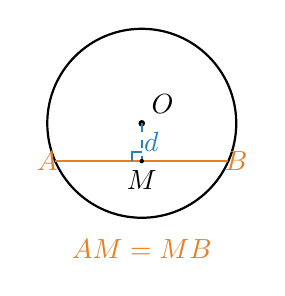
\begin{tikzpicture}[scale=0.8]
      \draw[thick] (0,0) circle (1.5);
      \fill (0,0) circle (1.5pt) node[above right] {$O$};

      % Chord: horizontal at y=-0.6, half-length = sqrt(1.5²-0.6²)=1.374
      \draw[boxOrange, thick] (-1.374,-0.6) -- (1.374,-0.6);
      \node[boxOrange] at (-1.5,-0.6) {$A$};
      \node[boxOrange] at (1.5,-0.6) {$B$};

      % Perpendicular from center
      \draw[boxBlue, thick, dashed] (0,0) -- (0,-0.6);
      \node[boxBlue] at (0.15,-0.3) {$d$};

      % Midpoint marker
      \node at (0,-0.9) {$M$};
      \fill (0,-0.6) circle (1pt);

      % Right angle
      \draw[boxBlue, thick] (-0.15,-0.6) -- (-0.15,-0.45) -- (0,-0.45);

      % Labels
      \node[boxOrange] at (0,-2) {$AM = MB$};
    \end{tikzpicture}
  \end{center}

  \begin{exambox}
    $AM^2 + d^2 = r^2$ \quad (โดยทฤษฎีบทพีทาโกรัส)

    ถ้าทราบ $r = 5$, $AB = 8$ จะได้ $AM = 4$, $d = \sqrt{5^2 - 4^2} = 3$
  \end{exambox}
\end{frame}

\begin{frame}{คอร์ดที่เท่ากัน}
  \begin{explanation}[ทฤษฎีบทที่ 2]
    \textbf{ในวงกลมเดียวกันหรือวงกลมที่เท่ากันทุกประการ:}
    \begin{enumerate}
      \item คอร์ดที่เท่ากันจะอยู่ห่างจากจุดศูนย์กลางเท่ากัน
      \item คอร์ดที่อยู่ห่างจากจุดศูนย์กลางเท่ากันจะยาวเท่ากัน
    \end{enumerate}
  \end{explanation}

  \begin{center}
    \begin{tikzpicture}[scale=1]
      \draw[thick] (0,0) circle (1.5);
      \fill (0,0) circle (1.2pt) node[below left] {$O$};

      % Chord 1: horizontal at y=0.9, half-length=sqrt(2.25-0.81)=1.2
      \draw[boxBlue, thick] (-1.2,0.9) -- (1.2,0.9);
      \draw[boxBlue, dashed] (0,0) -- (0,0.9);
      % Right angle at midpoint: chord direction=0°, perp=90°
      \draw[boxBlue, thick] (0.1,0.9) -- (0.1,0.78) -- (0,0.78);
      \node[boxBlue] at (0.12,0.45) {$d_1$};

      \draw[boxOrange, thick] (-1.2,-0.9) -- (1.2,-0.9);
      \draw[boxOrange, dashed] (0,0) -- (0,-0.9);
      % Right angle at midpoint
      \draw[boxOrange, thick] (0.1,-0.9) -- (0.1,-0.78) -- (0,-0.78);
      \node[boxOrange] at (0.12,-0.45) {$d_2$};

      \node at (0,-2) {$d_1 = d_2 \;\Longleftrightarrow\;$ คอร์ดยาวเท่ากัน};
    \end{tikzpicture}
  \end{center}
\end{frame}

% ===========================================================================
%  SECTION 3: เส้นสัมผัสวงกลม
% ===========================================================================
\section{เส้นสัมผัสวงกลม (Tangents to a Circle)}

\begin{frame}{สมบัติของเส้นสัมผัส}
  \begin{explanation}[ทฤษฎีบท]
    \textbf{เส้นสัมผัสวงกลมจะตั้งฉากกับรัศมีที่จุดสัมผัส}
  \end{explanation}

  \begin{center}
    \begin{tikzpicture}[scale=1]
      \draw[thick] (0,0) circle (1.5);
      \fill (0,0) circle (1.2pt) node[below right] {$O$};

      % Radius to tangent point at right
      \draw[boxBlue, thick] (0,0) -- (1.5,0) node[midway, below] {$r$};

      % Tangent line at (1.5,0) — vertical
      \draw[boxOrange, thick] (1.5,-1.5) -- (1.5,1.5);
      \node[boxOrange] at (1.5,1.7) {เส้นสัมผัส};

      % Right angle marker
      \draw[boxBlue, thick] (1.2,0) -- (1.2,0.3) -- (1.5,0.3);

      % Touch point
      \fill (1.5,0) circle (1.2pt) node[above right] {$P$};
    \end{tikzpicture}
  \end{center}

  \begin{intuition}[ทำไมถึงตั้งฉาก?]
    ถ้าไม่ตั้งฉาก รัศมีจะไม่ใช่ระยะที่สั้นที่สุดจาก $O$ ไปเส้นสัมผัส
    แสดงว่าเส้นจะตัดวงกลม ขัดแย้งกับการเป็นเส้นสัมผัส
  \end{intuition}
\end{frame}

\begin{frame}{เส้นสัมผัสสองเส้นจากจุดภายนอก}
  \begin{explanation}[ทฤษฎีบท]
    \textbf{เส้นสัมผัสสองเส้นที่ลากจากจุดภายนอกวงกลม จะมีความยาวเท่ากัน}
    และเส้นที่เชื่อมจุดศูนย์กลางกับจุดภายนอกจะแบ่งครึ่งมุมระหว่างเส้นสัมผัสทั้งสอง
  \end{explanation}

  \begin{center}
    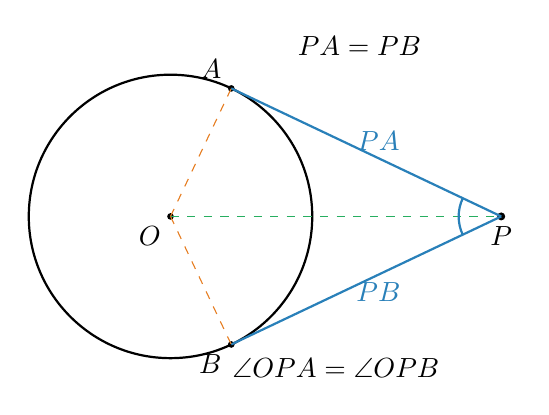
\begin{tikzpicture}[scale=1.2]
      \draw[thick] (0,0) circle (1.5);
      \fill (0,0) circle (1pt) node[below left] {$O$};

      % External point
      \fill (3.5,0) circle (1.2pt) node[below] {$P$};

      % Tangent points: cos α = r/OP = 1.5/3.5, α = 64.62°
      % tan pt = 1.5*(cos α, ±sin α) = (0.643, ±1.355)
      \fill (0.643,1.355) circle (1pt) node[above left] {$A$};
      \fill (0.643,-1.355) circle (1pt) node[below left] {$B$};

      % Tangents
      \draw[boxBlue, thick] (3.5,0) -- (0.643,1.355);
      \draw[boxBlue, thick] (3.5,0) -- (0.643,-1.355);

      % Radii
      \draw[boxOrange, dashed] (0,0) -- (0.643,1.355);
      \draw[boxOrange, dashed] (0,0) -- (0.643,-1.355);

      % Center to P
      \draw[boxGreen, dashed] (0,0) -- (3.5,0);

      % Angle at P: PA dir ≈ 154.6°, PB dir ≈ -154.6° (205.4°)
      % Arc centered at P, radius 0.45, from 154.6° to 205.4°
      \draw[boxBlue, thick] (3.093,0.192) arc (154.6:205.4:0.45);

      % Labels
      \node[boxBlue] at (2.2,0.8) {$PA$};
      \node[boxBlue] at (2.2,-0.8) {$PB$};
      \node at (2.0,1.8) {$PA = PB$};
      \node at (1.75,-1.6) {$\angle OPA = \angle OPB$};
    \end{tikzpicture}
  \end{center}
\end{frame}

\begin{frame}{ทฤษฎีบทมุมระหว่างเส้นสัมผัสและคอร์ด}
  \begin{explanation}[Alternate Segment Theorem]
    \textbf{มุมระหว่างเส้นสัมผัสกับคอร์ดที่จุดสัมผัส
    เท่ากับมุมในส่วนโค้งตรงข้าม (Alternate Segment)}
  \end{explanation}

  \begin{center}
    \begin{tikzpicture}[scale=1.2]
      \draw[thick] (0,0) circle (1.5);
      \fill (0,0) circle (1pt) node[below left] {$O$};

      % A at top (90°), B at left (180°)
      \fill (0,1.5) circle (1pt) node[above] {$A$};
      \fill (-1.5,0) circle (1pt) node[below left] {$B$};

      % Tangent at A: perpendicular to OA (90°), so tangent is horizontal
      \draw[boxOrange, thick] (-1.5,1.5) -- (1.2,1.5);
      \node[boxOrange] at (1.5,1.5) {เส้นสัมผัส};

      % Chord AB
      \draw[boxBlue, thick] (0,1.5) -- (-1.5,0);

      % Angle between tangent (180° or 0°) and chord (toward B, dir 225°)
      % Tangent going leftward = 180°, chord direction = 225°, angle = 45°
      \draw[boxBlue, thick] (-0.35,1.5) arc (180:225:0.35);
      \node[boxBlue] at (-0.2,1.1) {$\alpha$};

      % C on alternate segment (right-lower quadrant)
      \fill (1.061,-1.061) circle (1pt) node[right] {$C$};

      % Lines AC and BC
      \draw[boxGreen, thin] (0,1.5) -- (1.061,-1.061);
      \draw[boxGreen, thin] (-1.5,0) -- (1.061,-1.061);

      % Angle at C: CA dir ~112.5°, CB dir ~157.5°, diff = 45°
      \draw[boxGreen, thick] (0.927,-0.738) arc (112.5:157.5:0.35);
      \node[boxGreen] at (0.7,-1.1) {$\alpha$};

      \node at (0,-1.8) {มุมระหว่างคอร์ด $AB$ กับเส้นสัมผัสที่ $A$ = มุมในส่วนโค้งตรงข้าม};
    \end{tikzpicture}
  \end{center}
\end{frame}

% ===========================================================================
%  SECTION 4: มุมในวงกลม
% ===========================================================================
\section{มุมในวงกลม (Angles in a Circle)}

\begin{frame}{มุมที่จุดศูนย์กลางและมุมในส่วนโค้ง}
  \begin{explanation}[Central Angle Theorem]
    \textbf{มุมที่จุดศูนย์กลางมีขนาดเป็น 2 เท่าของมุมในส่วนโค้ง ที่รองรับด้วยส่วนโค้งเดียวกัน}

    \[
      \angle AOB = 2\;\angle ACB
    \]
  \end{explanation}

  \begin{center}
    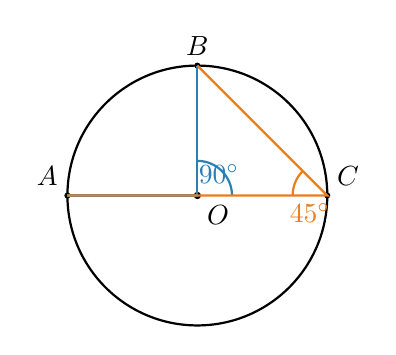
\begin{tikzpicture}[scale=1.1]
      \draw[thick] (0,0) circle (1.5);
      \fill (0,0) circle (1.2pt) node[below right] {$O$};

      % A = left, B = top, C = right
      \fill (-1.5,0) circle (1pt) node[above left] {$A$};
      \fill (0,1.5) circle (1pt) node[above] {$B$};
      \fill (1.5,0) circle (1pt) node[above right] {$C$};

      % Central angle AOB
      \draw[boxBlue, thick] (-1.5,0) -- (0,0) -- (0,1.5);
      \draw[boxBlue, thick] (0.4,0) arc (0:90:0.4);
      \node[boxBlue] at (0.25,0.25) {$90^\circ$};

      % Inscribed angle ACB
      \draw[boxOrange, thick] (-1.5,0) -- (1.5,0) -- (0,1.5);
      \draw[boxOrange, thick] (1.1,0) arc (180:135:0.4);
      \node[boxOrange] at (1.3,-0.2) {$45^\circ$};
    \end{tikzpicture}
  \end{center}
  \qquad $\angle AOB = 2\;\angle ACB$
\end{frame}

\begin{frame}{มุมในครึ่งวงกลม (Thales' Theorem)}
  \begin{explanation}[ทฤษฎีบท]
    \textbf{มุมในครึ่งวงกลมเป็นมุมฉากเสมอ} — มุมที่อยู่บนเส้นรอบวงและรองรับด้วยเส้นผ่านศูนย์กลางจะเท่ากับ $90^\circ$
  \end{explanation}

  \begin{center}
    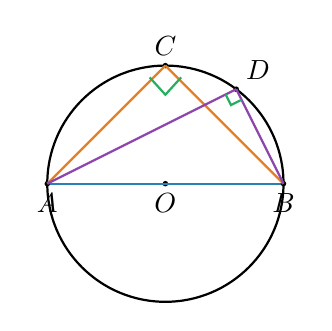
\begin{tikzpicture}[scale=1]
      \draw[thick] (0,0) circle (1.5);
      \fill (0,0) circle (1pt) node[below] {$O$};

      \draw[boxBlue, thick] (-1.5,0) -- (1.5,0);
      \fill (-1.5,0) circle (1pt) node[below] {$A$};
      \fill (1.5,0) circle (1pt) node[below] {$B$};

      \fill (0,1.5) circle (1pt) node[above] {$C$};
      \draw[boxOrange, thick] (0,1.5) -- (-1.5,0);
      \draw[boxOrange, thick] (0,1.5) -- (1.5,0);
      \draw[boxGreen, thick] (-0.2,1.35) -- (0,1.13) -- (0.2,1.35);

      \fill (0.9,1.2) circle (1pt) node[above right] {$D$};
      \draw[boxPurple, thick] (0.9,1.2) -- (-1.5,0);
      \draw[boxPurple, thick] (0.9,1.2) -- (1.5,0);
      % Right angle at D: DB dir ~296.6°, DA dir ~206.6°, leg=0.15
      \draw[boxGreen, thick] (0.967,1.066) -- (0.833,0.999) -- (0.766,1.133);
    \end{tikzpicture}
  \end{center}

  \begin{intuition}[บทกลับ]
    ถ้าสามเหลี่ยมมีมุมฉาก ด้านตรงข้ามมุมฉากจะเป็นเส้นผ่านศูนย์กลางของวงกลมล้อมรอบ
  \end{intuition}
\end{frame}

\begin{frame}{มุมในส่วนโค้งเดียวกัน}
  \begin{explanation}[ทฤษฎีบท]
    \textbf{มุมในส่วนโค้งเดียวกัน (ที่รองรับด้วยคอร์ดเดียวกัน) จะมีขนาดเท่ากัน}
    \[
      \angle ACB = \angle ADB = \angle AEB
    \]
  \end{explanation}

  \begin{center}
    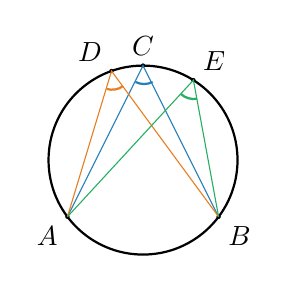
\begin{tikzpicture}[scale=0.8]
      \draw[thick] (0,0) circle (1.5);

      % Chord AB at bottom
      \fill (-1.2,-0.9) circle (1pt) node[below left] {$A$};
      \fill (1.2,-0.9) circle (1pt) node[below right] {$B$};

      % Three points on upper arc
      \fill (0,1.5) circle (1pt) node[above] {$C$};
      \fill (-0.5,1.414) circle (1pt) node[above left] {$D$};
      \fill (0.8,1.269) circle (1pt) node[above right] {$E$};

      % Lines and angle arcs at C, D, E (inscribed angles ≈ 53°, all equal)
      \draw[boxBlue, thin] (-1.2,-0.9) -- (0,1.5) -- (1.2,-0.9);
      \draw[boxBlue, thick] (-0.12,1.24) arc (-117:-63:0.3);

      \draw[boxOrange, thin] (-1.2,-0.9) -- (-0.5,1.414) -- (1.2,-0.9);
      \draw[boxOrange, thick] (-0.58,1.13) arc (-107:-54:0.3);

      \draw[boxGreen, thin] (-1.2,-0.9) -- (0.8,1.269) -- (1.2,-0.9);
      \draw[boxGreen, thick] (0.60,1.05) arc (-133:-80:0.3);
    \end{tikzpicture}
  \end{center}

  \begin{intuition}[จำง่าย ๆ]
    มองหาคอร์ดร่วม แล้วหามุมอื่นที่รองรับด้วยคอร์ดเดียวกัน — มุมในส่วนโค้งเดียวกันย่อมเท่ากัน
  \end{intuition}
\end{frame}

\begin{frame}{ตัวอย่าง: มุมในวงกลม}
  \begin{exambox}[โจทย์]
    จากรูป $O$ เป็นจุดศูนย์กลาง $\angle AOB = 80^\circ$ จงหา $\angle ACB$
  \end{exambox}

  \begin{columns}[T]
    \column{0.45\textwidth}
      \centering
      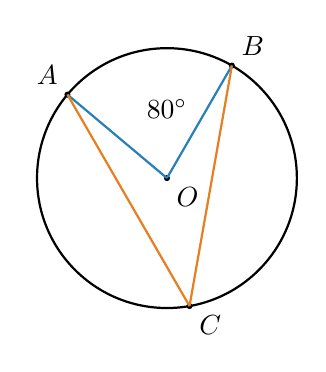
\begin{tikzpicture}[scale=1.1]
        \draw[thick] (0,0) circle (1.5);
        \fill (0,0) circle (1pt) node[below right] {$O$};

        \fill (140:1.5) circle (1pt) node[above left] {$A$};
        \fill (60:1.5) circle (1pt) node[above right] {$B$};
        \fill (-80:1.5) circle (1pt) node[below right] {$C$};

        \draw[boxBlue, thick] (0,0) -- (140:1.5);
        \draw[boxBlue, thick] (0,0) -- (60:1.5);
        \draw[boxOrange, thick] (140:1.5) -- (-80:1.5);
        \draw[boxOrange, thick] (60:1.5) -- (-80:1.5);

        \node at (0,0.8) {$80^\circ$};
      \end{tikzpicture}

    \column{0.55\textwidth}
      \begin{solbox}[วิธีทำ]
        $\angle AOB = 80^\circ$ (มุมที่จุดศูนย์กลาง)

        $\angle ACB$ รองรับส่วนโค้ง $AB$ เดียวกัน

        \[
          \angle ACB = \tfrac{1}{2} \times 80^\circ = 40^\circ
        \]
      \end{solbox}
  \end{columns}
\end{frame}

% ===========================================================================
%  SECTION 5: รูปสี่เหลี่ยมแนบในวงกลม
% ===========================================================================
\section{รูปสี่เหลี่ยมแนบในวงกลม (Cyclic Quadrilateral)}

\begin{frame}{นิยามและสมบัติ}
  \begin{explanation}[นิยาม]
    \textbf{รูปสี่เหลี่ยมแนบในวงกลม (Cyclic Quadrilateral)} คือรูปสี่เหลี่ยมที่มีจุดยอดทั้งสี่อยู่บนเส้นรอบวงของวงกลมเดียวกัน
  \end{explanation}

  \begin{center}
    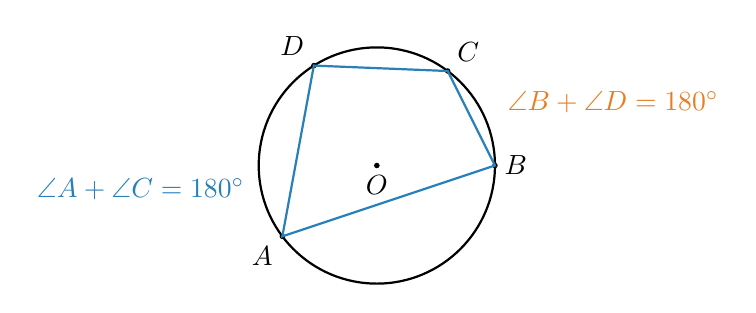
\begin{tikzpicture}[scale=1]
      \draw[thick] (0,0) circle (1.5);
      \fill (0,0) circle (1pt) node[below] {$O$};

      \fill (-1.2,-0.9) circle (1pt) node[below left] {$A$};
      \fill (1.5,0) circle (1pt) node[right] {$B$};
      \fill (0.9,1.2) circle (1pt) node[above right] {$C$};
      \fill (-0.8,1.269) circle (1pt) node[above left] {$D$};

      \draw[boxBlue, thick] (-1.2,-0.9) -- (1.5,0) -- (0.9,1.2) -- (-0.8,1.269) -- cycle;

      \node[boxBlue] at (-3,-0.3) {$\angle A + \angle C = 180^\circ$};
      \node[boxOrange] at (3,0.8) {$\angle B + \angle D = 180^\circ$};
    \end{tikzpicture}
  \end{center}

  \begin{explanation}
    \textbf{มุมตรงข้ามรวมกัน $= 180^\circ$}: \;
    $\angle A + \angle C = 180^\circ$, \;
    $\angle B + \angle D = 180^\circ$

    \textbf{มุมภายนอก $=$ มุมภายในที่อยู่ตรงข้าม}
  \end{explanation}
\end{frame}

\begin{frame}{บทกลับ — ทดสอบว่าแนบในวงกลมได้หรือไม่}
  \begin{explanation}[บทกลับ]
    รูปสี่เหลี่ยมจะแนบในวงกลมได้ \textbf{ก็ต่อเมื่อ} มุมตรงข้ามรวมกัน $= 180^\circ$

    \medskip
    หรือกล่าวอีกแบบ: มุมภายนอกที่จุดยอดหนึ่ง $=$ มุมภายในที่จุดยอดตรงข้าม
  \end{explanation}

  \begin{center}
    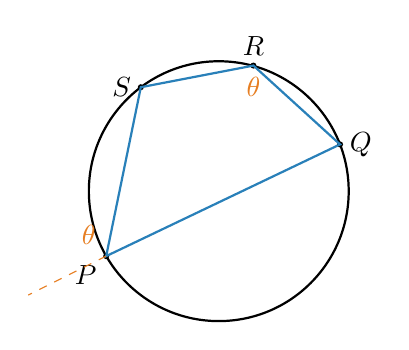
\begin{tikzpicture}[scale=1.1]
      \draw[thick] (0,0) circle (1.5);

      \fill (-1.3,-0.75) circle (1pt) node[below left] {$P$};
      \fill (1.4,0.54) circle (1pt) node[right] {$Q$};
      \fill (0.4,1.45) circle (1pt) node[above] {$R$};
      \fill (-0.9,1.2) circle (1pt) node[left] {$S$};

      \draw[boxBlue, thick] (-1.3,-0.75) -- (1.4,0.54) -- (0.4,1.45) -- (-0.9,1.2) -- cycle;

      \draw[boxOrange, dashed] (-1.3,-0.75) -- (-2.2,-1.2);
      \node[boxOrange] at (-1.5,-0.5) {$\theta$};
      \node[boxOrange] at (0.4,1.2) {$\theta$};
    \end{tikzpicture}
  \end{center}
\end{frame}

\begin{frame}{ตัวอย่าง: รูปสี่เหลี่ยมแนบใน}
  \begin{exambox}[โจทย์]
    รูปสี่เหลี่ยม $ABCD$ แนบในวงกลม $\angle A = 95^\circ$, $\angle B = 70^\circ$ จงหา $\angle C$ และ $\angle D$
  \end{exambox}

  \begin{solbox}[วิธีทำ]
    \begin{align*}
      \angle A + \angle C &= 180^\circ \;\Rightarrow\; \angle C = 180^\circ - 95^\circ = 85^\circ \\[4pt]
      \angle B + \angle D &= 180^\circ \;\Rightarrow\; \angle D = 180^\circ - 70^\circ = 110^\circ
    \end{align*}
  \end{solbox}
\end{frame}

\begin{frame}{ตัวอย่าง: รูปสี่เหลี่ยมแนบใน (ต่อ)}
  \begin{exambox}[โจทย์]
    $ABCD$ แนบในวงกลม โดย $\angle ABC = 2\angle ADC$ จงหา $\angle ADC$
  \end{exambox}

  \begin{solbox}[วิธีทำ]
    $\angle ABC + \angle ADC = 180^\circ$

    $2\angle ADC + \angle ADC = 180^\circ \;\Rightarrow\; 3\angle ADC = 180^\circ \;\Rightarrow\; \angle ADC = 60^\circ$
  \end{solbox}

  \begin{intuition}[เทคนิค]
    ตั้งสมการจากสมบัติมุมตรงข้ามรวมกันได้ $180^\circ$ แล้วแก้หาค่ามุมที่ต้องการ
  \end{intuition}
\end{frame}

% ===========================================================================
%  SECTION 6: ตัวอย่างโจทย์ประยุกต์
% ===========================================================================
\section{ตัวอย่างโจทย์ประยุกต์}

\begin{frame}{ตัวอย่าง: เส้นสัมผัสและสี่เหลี่ยมแนบใน}
  \begin{exambox}[โจทย์]
    $PA$ และ $PB$ เป็นเส้นสัมผัสวงกลมที่ลากจาก $P$
    $\angle APB = 50^\circ$ จงหา $\angle AOB$
  \end{exambox}

  \begin{columns}[T]
    \column{0.45\textwidth}
      \centering
      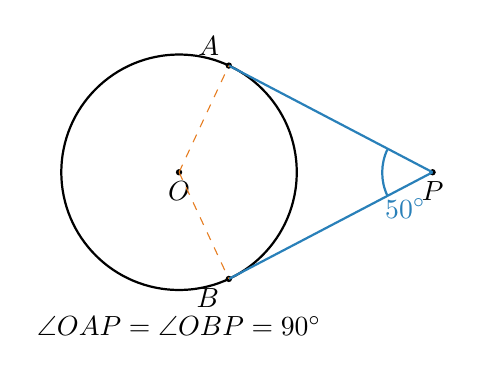
\begin{tikzpicture}[scale=1.15]
        \draw[thick] (0,0) circle (1.3);
        \fill (0,0) circle (1pt) node[below] {$O$};

        \fill (2.8,0) circle (1pt) node[below] {$P$};

        % Tangent points
        \fill (0.55,1.178) circle (1pt) node[above left] {$A$};
        \fill (0.55,-1.178) circle (1pt) node[below left] {$B$};

        % Tangents
        \draw[boxBlue, thick] (2.8,0) -- (0.55,1.178);
        \draw[boxBlue, thick] (2.8,0) -- (0.55,-1.178);

        % Radii
        \draw[boxOrange, dashed] (0,0) -- (0.55,1.178);
        \draw[boxOrange, dashed] (0,0) -- (0.55,-1.178);

        % Angle at P
        \draw[boxBlue, thick] (2.3,0.25) arc (155:205:0.6);
        \node[boxBlue] at (2.5,-0.4) {$50^\circ$};

        \node at (0,-1.7) {$\angle OAP = \angle OBP = 90^\circ$};
      \end{tikzpicture}

    \column{0.55\textwidth}
      \begin{solbox}[วิธีทำ]
        ในสี่เหลี่ยม $OAPB$:
        \begin{itemize}
          \item เส้นสัมผัส $\perp$ รัศมี: $\angle OAP = \angle OBP = 90^\circ$
          \item มุมภายในสี่เหลี่ยมรวมกัน $= 360^\circ$:
        \end{itemize}
        \begin{align*}
          90^\circ + 90^\circ + \angle AOB + 50^\circ &= 360^\circ \\
          \angle AOB &= 130^\circ
        \end{align*}
      \end{solbox}
  \end{columns}
\end{frame}

\begin{frame}{ตัวอย่าง: หามุมจากคอร์ดร่วม}
  \begin{exambox}[โจทย์]
    ในวงกลมวงหนึ่ง $AB$ เป็นคอร์ด $C$ และ $D$ เป็นจุดบนส่วนโค้งเดียวกันของ $AB$
    ถ้า $\angle ACB = 40^\circ$ จงหา $\angle ADB$
  \end{exambox}

  \begin{solbox}[วิธีทำ]
    $\angle ACB$ และ $\angle ADB$ ต่างก็รองรับด้วยคอร์ด $AB$ และอยู่บนส่วนโค้งเดียวกัน

    ดังนั้น $\angle ADB = \angle ACB = 40^\circ$

    \textbf{หลักการ:} มุมในส่วนโค้งเดียวกันย่อมเท่ากัน!
  \end{solbox}

  \begin{center}
    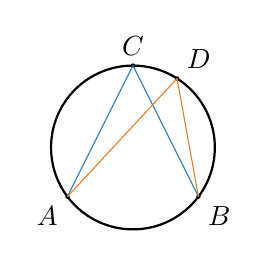
\begin{tikzpicture}[scale=0.8]
      \draw[thick] (0,0) circle (1.3);
      \fill (-1.04,-0.78) circle (1pt) node[below left] {$A$};
      \fill (1.04,-0.78) circle (1pt) node[below right] {$B$};
      \fill (0,1.3) circle (1pt) node[above] {$C$};
      \fill (0.7,1.095) circle (1pt) node[above right] {$D$};

      \draw[boxBlue] (-1.04,-0.78) -- (0,1.3) -- (1.04,-0.78);
      \draw[boxOrange] (-1.04,-0.78) -- (0.7,1.095) -- (1.04,-0.78);
    \end{tikzpicture}
  \end{center}
\end{frame}

% ===========================================================================
%  SUMMARY
% ===========================================================================
\section{สรุป}

\begin{frame}{สรุปเนื้อหา}
  \begin{explanation}[สิ่งที่ได้เรียนรู้]
    \begin{enumerate}
      \item \textbf{ส่วนประกอบวงกลม}: จุดศูนย์กลาง, รัศมี, คอร์ด, เส้นสัมผัส, เซกเตอร์
      \item \textbf{สูตรพื้นฐาน}: $C = 2\pi r$, $A = \pi r^2$, ความยาวส่วนโค้ง, พื้นที่เซกเตอร์
      \item \textbf{คอร์ด}: เส้นที่ลากจากจุดศูนย์กลางตั้งฉากกับคอร์ดจะแบ่งครึ่งคอร์ด
             — คอร์ดเท่ากันอยู่ห่างจากจุดศูนย์กลางเท่ากัน
      \item \textbf{เส้นสัมผัส}: ตั้งฉากกับรัศมี — เส้นสัมผัสจากจุดภายนอกยาวเท่ากัน
             — มุมระหว่างเส้นสัมผัสกับคอร์ด = มุมในส่วนโค้งตรงข้าม
      \item \textbf{มุมในวงกลม}: มุมที่จุดศูนย์กลาง $= 2\times$ มุมในส่วนโค้ง,
             มุมในครึ่งวงกลม $= 90^\circ$, มุมในส่วนโค้งเดียวกันเท่ากัน
      \item \textbf{สี่เหลี่ยมแนบใน}: มุมตรงข้ามรวมกัน $= 180^\circ$,
             มุมภายนอก $=$ มุมภายในตรงข้าม
    \end{enumerate}
  \end{explanation}
  \begin{center}
    \large เอกสารนี้เป็นส่วนหนึ่งของเนื้อหาเตรียมสอบ \textbf{สอวน. คอมพิวเตอร์}
  \end{center}
\end{frame}

\end{document}
